\documentclass{homework}

\usepackage{subfig}
\usepackage{multicol}
\usepackage{float}
\usepackage{bookmark}
\usepackage{hyperref}
\usepackage{xcolor}
\usepackage{listings}
\lstset{literate=
	{á}{{\'a}}1 {é}{{\'e}}1 {í}{{\'i}}1 {ó}{{\'o}}1 {ú}{{\'u}}1
	{Á}{{\'A}}1 {É}{{\'E}}1 {Í}{{\'I}}1 {Ó}{{\'O}}1 {Ú}{{\'U}}1
	{à}{{\`a}}1 {è}{{\`e}}1 {ì}{{\`i}}1 {ò}{{\`o}}1 {ù}{{\`u}}1
	{À}{{\`A}}1 {È}{{\'E}}1 {Ì}{{\`I}}1 {Ò}{{\`O}}1 {Ù}{{\`U}}1
	{ä}{{\"a}}1 {ë}{{\"e}}1 {ï}{{\"i}}1 {ö}{{\"o}}1 {ü}{{\"u}}1
	{Ä}{{\"A}}1 {Ë}{{\"E}}1 {Ï}{{\"I}}1 {Ö}{{\"O}}1 {Ü}{{\"U}}1
	{â}{{\^a}}1 {ê}{{\^e}}1 {î}{{\^i}}1 {ô}{{\^o}}1 {û}{{\^u}}1
	{Â}{{\^A}}1 {Ê}{{\^E}}1 {Î}{{\^I}}1 {Ô}{{\^O}}1 {Û}{{\^U}}1
	{ã}{{\~a}}1 {ẽ}{{\~e}}1 {ĩ}{{\~i}}1 {õ}{{\~o}}1 {ũ}{{\~u}}1
	{Ã}{{\~A}}1 {Ẽ}{{\~E}}1 {Ĩ}{{\~I}}1 {Õ}{{\~O}}1 {Ũ}{{\~U}}1
	{œ}{{\oe}}1 {Œ}{{\OE}}1 {æ}{{\ae}}1 {Æ}{{\AE}}1 {ß}{{\ss}}1
	{ű}{{\H{u}}}1 {Ű}{{\H{U}}}1 {ő}{{\H{o}}}1 {Ő}{{\H{O}}}1
	{ç}{{\c c}}1 {Ç}{{\c C}}1 {ø}{{\o}}1 {å}{{\r a}}1 {Å}{{\r A}}1
	{€}{{\euro}}1 {£}{{\pounds}}1 {«}{{\guillemotleft}}1
	{»}{{\guillemotright}}1 {ñ}{{\~n}}1 {Ñ}{{\~N}}1 {¿}{{?`}}1 {¡}{{!`}}1 
}

\definecolor{codegreen}{rgb}{0,0.6,0}
\definecolor{codegray}{rgb}{0.5,0.5,0.5}
\definecolor{codepurple}{rgb}{0.58,0,0.82}
\definecolor{backcolour}{rgb}{0.95,0.95,0.95}

\lstdefinestyle{mystyle}{
	backgroundcolor=\color{backcolour},   
	commentstyle=\color{codegreen},
	keywordstyle=\color{blue},
	numberstyle=\tiny\color{codegray},
	stringstyle=\color{codepurple},
	basicstyle=\ttfamily\footnotesize,
	breakatwhitespace=false,         
	breaklines=true,                 
	captionpos=b,                    
	keepspaces=true,                 
	numbers=left,                    
	numbersep=5pt,                  
	showspaces=false,                
	showstringspaces=false,
	showtabs=false,                  
	tabsize=2,
	xleftmargin=.25in
}

\lstset{style=mystyle}

\title{Práctica 1: Análisis de Eficiencia de Algoritmos}
\author{Shao Jie Hu Chen \\ Mario Megías Mateo \\ Jesús Samuel García Carballo}
\renewcommand{\course}{Algorítmica}
\date{1 de abril de 2022}

\begin{document}
	\maketitle

    \newpage

    \begin{abstract}
		Esto es una prueba
	\end{abstract}
	
    \newpage

	\tableofcontents
	\newpage
	\setcounter{page}{1}
	
	\section{Introducción}

    En esta primera práctica de la asignatura Algorítmica vamos a realizar un análisis teórico y empírico de
    diversos algoritmos vistos en la asignatura. En particular, dicho análisis se hará de los siguientes:

    \begin{itemize}
        \item \textbf{Algoritmos de ordenación:} Inserción, selección, quicksort y mergesort. 
        \item \textbf{Algoritmo de análisis de caminos mínimos sobre grafos:} Algoritmo de Floyd.
        \item \textbf{Hanoi.} Resolución del juego de las torres de Hanoi. 
    \end{itemize}

    \subsection{Estructura de la memoria}
    
	Esta memoria presenta la estructura típica de un trabajo académico. En primer lugar, presentamos
    brevemente el contexto en el que nos manejamos en esta práctica. Posteriormente, analizaremos teóricamente
    cada uno de los algoritmos propuestos para, seguidamente, comprobar mediante un 
    análisis empírico las soluciones obtenidas. Asimismo, se ha realizado un análisis híbrido contrastando
    los resultados teóricos con los experimentales. Este análisis se ha realizado para cada algoritmo, 
    extrayéndose información relevante asociada a ellas. 
    
    Además, para cada uno de los algoritmos considerados, se ha
    elaborado conjuntamente entre los miembros del grupo tablas asociadas a cada una de ellas, que se
    irán presentando a lo largo de esta memoria. Finalmente, se escribirán unas
    líneas asociadas a las conclusiones obtenidas tras el desarrollo de esta práctica, así como los resultados
    más relevantes obtenidos. 

    \subsection{Objetivos} 

    Entre los objetivos que vamos a realizar asociadas a esta práctica, caben destacar los siguientes: 

    \begin{itemize}
        \item \textbf{Estudio teórico, empírico e híbrido} y \textbf{comparación} de los algoritmos de ordenación más empleados, verificando los resultados teóricos.
        \item \textbf{Estudio teórico, empírico e híbrido} de algoritmos de alta complejidad, poniendo especial énfasis en su \textbf{viabilidad} en diferentes equipos. 
        \item Estudio del \textbf{aumento de eficiencia} de un mismo algoritmo para diferentes \textbf{tipos de optimización} del compilador. 
        \item Determinación del algoritmo \textbf{más adecuado} para cada situación en función del estado de los datos.
    \end{itemize}

    \subsection{Equipo empleado}

    Para el desarrollo de esta práctica, se han empleado diferentes equipos, cuyas respectivas especificaciones técnicas se 
    especifican a continuación:
    
    \begin{itemize}
        \item \textbf{ASUS} 
        \begin{itemize}
            \item \textbf{Modelo}: ZenBook 15 UX534F
            \item \textbf{Procesador}: Intel(R) Core(TM) i7-10510U CPU @ 1.80GHz5
            \item \textbf{Memoria Ram}: 16 GB DDR4 @ 2.133 MHz.
            \item \textbf{Sistema Operativo} Ubuntu 20.04.2 LTS
        \end{itemize}
        
        \item \textbf{LENOVO}
        \begin{itemize}
            \item \textbf{Modelo}: YOGA 530-14IKB
            \item \textbf{Procesador}: Intel(R) Core(TM) i5-8250U CPU @ 1.60GHz
            \item \textbf{Memoria RAM:} 8 GB DDR4
            \item \textbf{Sistema Operativo}: Ubuntu 20.04.4 LTS
        \end{itemize}
        
        \item \textbf{HP}
        \begin{itemize}
            \item \textbf{Modelo}: HP Pavilion Gaming Laptop 15-dk0xxx
            \item \textbf{Procesador}: Intel(R) Core(TM) i7-9750H CPU @ 2.60GHz
            \item \textbf{Memoria RAM:} 32 GB DDR4
            \item \textbf{Sistema Operativo}: Ubuntu 20.04.4 LTS
        \end{itemize}
    \end{itemize}
    

    \section{Metodología}

    Debido a las limitaciones técnicas de estos equipos, para el cálculo de la eficiencia empírica se ha 
    optado por medir tiempos de ejecución en tiempos y \textbf{tamaños razonables} para obtener datos relevantes
    para el comportamiento tanto a pequeñas escalas como a nivel asintótico de ellas. 

    Con el fin de automatizar el desarrollo de esta práctica, se ha diseñado un proyecto a la que hemos llamado 
    \textbf{GraphKiller}. Se trata de un conjunto de 6 scripts cuya última finalidad es la de automatizar la generación
    de los parámetros que aparecen en este práctica. Un esquema de este proyecto puede encontrar en la 
    figura \ref{graph-killer}. 

    \begin{figure}[H]
        \centering
        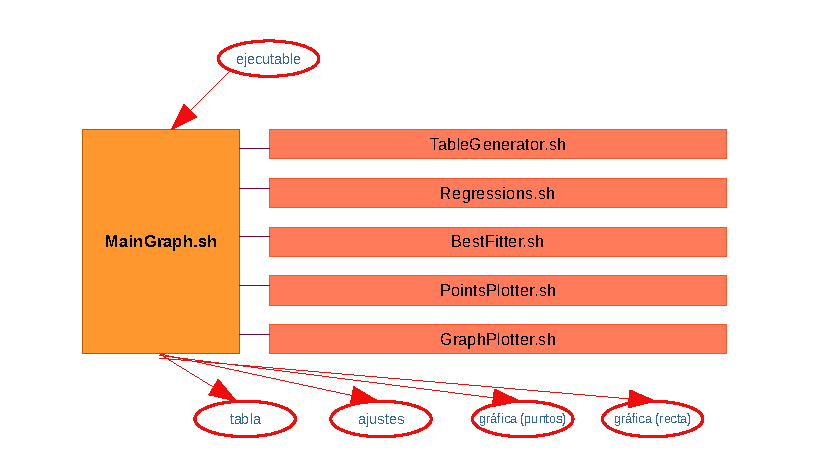
\includegraphics[width=0.9\textwidth]{img/esquema_graphkiller.pdf}
        \caption{Esquema del funcionamiento de GraphKiller}
        \label{graph-killer}
    \end{figure}

    Consta de las siguientes partes:

    \begin{enumerate}
        \item \textbf{TableGenerator.sh}. Se encarga de generar las tablas de datos, teniendo en cuenta número de repeticiones, valores iniciales y finales y cantidad de medidas experimentales a tomar.
        \item \textbf{Regressions.sh}. Se encarga de generar una lista de las regresiones más empleadas en Algorítmica, dando información como función de ajuste y parámetros estadísticos como la varianza residual de la regresión.
        \item \textbf{BestFitter.sh}. Su labor es la de escoger siempre la regresión que mejor se ajusta (con menor varianza residual). Presenta el inconveniente de que no sabe discriminar los datos, únicamente compara residuos.
        \item \textbf{PointsPlotter.sh}. Produce un gráfico con los puntos de la tabla de datos obtenida.
        \item \textbf{GraphPlotter.sh}. Produce un gráfico con los puntos de la tabla de datos obtenida, así como la curva de regresión óptima. 
    \end{enumerate}

    \section{Eficiencia teórica}

    Para el análisis de los siguientes algoritmos se ha empleado la notación $O(.)$. 

    \subsection{Algoritmo de inserción}

    El código de este algoritmo lo podemos encontrar a continuación.

    \lstinputlisting[language=C++, firstline=66, lastline=79, caption=Implementación en C++ del algoritmo de inserción.]{../src/insercion.cpp}
    
    El análisis de eficiencia se ha de hacer sobre el número de elementos del vector $n$. 

    Para el análisis asintótico, calculamos el número de operaciones elementales asociadas al código. 
    Las tres primeras líneas tienen complejidad $O(1)$. Para el ciclo for, démonos cuenta de que itera sobre el número de
    componentes del vector. Por su parte, dentro del for existe un while que realiza un conjunto de operaciones de orden
    $O(1)$ tantas veces como se indica en el iterador. Por tanto, llamando $T(n)$ al números de operaciones asociadas
    al algoritmo, tenemos que:

    \begin{equation*}
        T(n) = \sum_{i=0}^{n-1} \sum_{j=0}^{i-1} k = \sum_{i=0}^{n-1} ki = k \frac{n(n-1)}{2} 
    \end{equation*}

    Por tanto, deducimos que $T(n) \in O(n^2)$. 

    \subsection{Algoritmo de selección}

    \lstinputlisting[language=C++, firstline=66, lastline=82, caption=Implementación en C++ del algoritmo de selección.]{../src/seleccion.cpp}    

    La estructura principal del código anterior consta de dos bucles for anidados. Las primeras sentencias de declaración antes del inicio del primer 
    bucle for no repercuten en el análisis. Procedamos a analizar la estructura repetitiva: el primer for recorre el vector desde su inicio hasta
    la penúltima componente del mismo incluída. El segundo for comienza en la posición dada por el índice del primero hasta la última componente del vector incluída.
    Dentro del bucle interno tenemos una operación elemental correspondiente a la comparación realizada en el if, que es $O(1)$. Dentro del bucle externo excluyendo 
    el código del bucle interno nos encontramos con dos sentencias de asignación que no se tendrán en cuenta para el análisis. De igual modo, fuera del bucle externo
    al final del código nos encontramos con otras sentencias de asignación que también serán despreciadas. También tendremos en cuenta las operaciones elementales
    aritméticos correspondientes a la gestión de los bucles, que son $O(1)$. En conclusion, acotando las expresiones $O(1)$ por k tenemos que: 

    \begin{equation*}
        \begin{split}
            T(n) = \sum_{i=0}^{n-2} \sum_{j=i}^{n-1} k = \sum_{i=0}^{n-2} k(n-1-i+1) = \sum_{i=0}^{n-2} k(n-i) = kn \sum_{i=0}^{n-2} 1  - k \sum_{i=0}^{n-2} i \\
            = kn(n-2+1) - k \frac{(n-2)(n-1)}{2} = kn^2 + kn - \frac{kn^2 - 3kn + 2k}{2}
        \end{split}
    \end{equation*}
    
    Deducimos, por tanto, que $T(n) \in O(n^2)$. 
    
    \subsection{Algoritmo HeapSort}
    
    \lstinputlisting[language=C++, firstline=59, lastline=71, caption=Implementación en C++ del algoritmo heapsort.]{../src/heapsort.cpp} 

    El heapsort es un algoritmo de ordenación por montículos que consta de dos bucles for independientes, que llaman a una función llamada reajustar.
    En la primera línea de código podemos encontrar una declaración de variable cuya eficiencia es $O(1)$ y luego los dos ciclos mencionados, que interan 
    sobre el número de elementos del vector que denotaremos por $n$, luego realizaremos la eficiencia en torno a este dato. Ambos ciclos son independientes, 
    así que vamos a analizar cada uno por separado y aplicando la regla del máximo nos quedaremos con el mayor.
    
    La función reajustar trata de imitar el uso de un árbol APO mediante vectores y recorrerlo insertando elementos, luego como en un árbol APO la inserción se 
    realiza con eficiencia $O(log_2(n))$. Así que llamando $T(n)$ al números de operaciones asociadas al algoritmo, tenemos lo siguiente:
    
    \begin{itemize}
        \item \textbf{Primer ciclo}
        \begin{equation*}
            T(n) = \sum_{i=0}^{n/2 + 1} log_2(i) = log_2(k) \in O(nlog(n))
        \end{equation*} 

        \item \textbf{Segundo ciclo}
            $$\sum_{i=2}^{n} \log_2(i) = \log_2(2) + ... + \log_2(n) = \log_2(n!) \in O(n \log_2(n))$$
        
        
    \end{itemize}

    En conclusión vemos que como tenemos que aplicar la regla del máximo y ambos ciclos tienen de eficiencia $O(nlog(n))$ podemos afirmar que esa es la eficiencia
    teórica del algoritmo, 

    \subsection{Algoritmo QuickSort}
    
    \lstinputlisting[language=C++, firstline=141, lastline=184, caption=Implementación en C++ del algoritmo QuickSort.]{../src/quicksort.cpp} 

    En este apartado, consideramos $n$ como el número de componentes del vector. 

    El código del algoritmo comienza en la función quicksort\_lims en la línea 6. Tomaremos inicial 
    como ñaa posición de comienzo del vector ($inicial = 0$), y final como el siguiente al último elemento, 
    que coincide con el número de componentes del vector ($final = n$).
    Tenemos una estructura condicional que determina el comportamiento del algoritmo según si el tamaño del vector 
    supera o no un cierto umbral, por lo que el tiempo de ejecución será una función definida a trozos. Si es menor 
    que el umbral, ejecutamos la ordenación con el algoritmo de inserción previamente analizado, que es $O(n^2)$. De lo
    contrario, realizamos la ordenación según el propio algoritmo quicksort. Dicho algoritmo se basa en la técnica de Divide
    y Vencerás, implementándose de forma recursiva. En primer lugar, se realiza una llamada a la función dividir dividir\_qs, 
    cuya eficiencia procedemos a analizar. En las líneas 24-26 y 40-43 tenemos sentencias de asignación que serán despreciadas. 
    Siguiendo código de forma secuencial, en las líneas 27 y 30 tenemos dos bucles do-while, si consideramos el peor caso para 
    el primero (el pivote es mayor que el resto de elemento) tiene eficiencia $O(n)$, y el caso contrario al anterior sería el 
    más desfavorable para el segundo (el pivote es menor que el resto de los elementos), luego tendríamos $O(n)$. Como el caso más 
    favorable para uno (eficiencia $O(1)$) es el más desfavorable para el otro, aplicando la regla del Máximo tenemos que la 
    eficiencia de la parte del código de los do-while sería $O(n)$.  A continuación, encontramos un bucle while que se ejecuta un 
    número indeterminado de veces en función de la condición, luego podemos acotar estas ejecuciones por una constante c. En las 
    líneas 34-36 tenemos sentencias de asignación que serán ignoradas, y a continuación dos bucles do-while con la misma funcionalidad
    que los analizados anteriormente. Por tanto, deducimos que la eficiencia del bucle while es $O(n)$, y aplicando la regla del 
    Máximo con el bloque de código de los bucles do-while obtenemos que la eficiencia de la función es $O(n)$. A continuación hacemos dos llamadas
    recursivas, una que procesará los datos desde el comienzo del mismo hasta la posición en la que hemos ubicado el pivote con la 
    función dividir\_qs, y la otra se encarga de procesar el resto del vector. Por tanto, el tiempo de ejecución sería:

    \begin{equation}
        T(n) = \left\{ \begin{array}{lr} T(k_n) + T(n-k_n) + n & \text{si } n \geq \text{UMBRAL}\\ n^2 & \text{si } n < \text{UMBRAL} \end{array} \right.
    \end{equation}

    Para el caso promedio, podemos considerar que $k_{n} = \frac{n}{2}$. Resolvamos la recurrencia de (1):
    
    \begin{equation}
        T(n) = T(k_n) + T(n-k_n) + n \text{ si n $\geq$ UMBRAL}
    \end{equation}

    Realizamos el cambio de variable $n = 2^{n}$ en la ecuación (2) obtenemos:

    \begin{equation}
        T(2^{m}) = 2T(2^{m-1}) + 2^{m} \text{ si n $\geq log_{2}$(UMBRAL)} 
    \end{equation}

    \begin{equation}
        T(2^{m}) - 2T(2^{m-1}) = 2^{m}
    \end{equation}

    Renombramos la expresión anterior como $T(2^{m}) = t_{m}$ obtenemos:

    \begin{equation}
        t_{m} - 2t_{m-1} = 2^{m}
    \end{equation}
    
    Obtenemos la siguiente ecuación de recurrencia de la ecuación (5):

    \begin{equation}
        (x-2)^{2} = 0
    \end{equation}

    Luego la solución general de la recurrencia es:

    \begin{equation}
        t_{m} = c_{1}2^{m} + c_{2}m2^{m}
    \end{equation}

    Deshacemos el cambio de variable:

    \begin{equation}
        T(n) = c_{1}n + c_{2}nlog_{2}(n)
    \end{equation}

    Por tanto $T(n) \in O(nlog_{2}(n))$ si n $\geq$ UMBRAL.
    
    \subsection{Algoritmo de Floyd}

    A continuación se presenta el código de este algoritmo:

    \lstinputlisting[language=C++, firstline=129, lastline=138, caption=Implementación en C++ del algoritmo de Floyd.]{../src/floyd.cpp}

    En este caso, consideramos como $n$ el número de filas/columnas de la matriz. Como los tres bucles iteran cada uno sobre n, siendo el número de iteraciones
    independientes entre sí y se realizan $k$ operaciones en cada una de ellas, tenemos que llamando $T(n)$ al número de operaciones para un tamaño n, se verifica:
    
    \begin{equation*}
        T(n) = \sum_{i=1}^n \sum_{j=1}^{n} \sum_{k=1}^{n} k = kn^3
    \end{equation*}

    Deducimos fácilmente que $T(n) \in O(n^3)$. 
    
    \subsection{Algoritmo Hanoi}
    
    \lstinputlisting[language=C++, firstline=30, lastline=38, caption=Implementación en C++ del algoritmo de resolución de las torres de Hanoi.]{../src/hanoi.cpp} 

    Estamos ante el estudio de un algoritmo recursivo, así que si T(n) es el número de movimientos necesarios para mover n discos, tenemos que el algoritmo sigue la 
    recurrencia $T(n) = 2T(n-1) + 1$ $\forall n \geq 1$ y con $T(0) = 0$ como caso base. Por lo tanto, vamos a resolverla para hallar su eficiencia teórica.

    Tenemos que $t_n - 2t_{n-1} = 1 $ luego si hacemos un cambio de varible nos queda como ecuación característica $(x-2)(x-1) = 0$, que son las propias raíces de la 
    recurrencia luego la solución nos queda $t_n = c_1 1^n  + c_2 2^n  $. Como $t_0=0$, nos sale que $t_0 = c_1 + c_2$ y $t_1 = 2 t_0 + 1 = 1$, luego en la 
    solución $t_1=c_1 + 2 c_2 $, de donde si resolvemos el sistema $c_1 = 1$ y $c_2 = -1$ nos queda la ecuación $2^n - 1^n$. 
    
    En consecuencia, deducimos que se trata de la ecuación que 
    modela la recurrencia, lo que nos permite concluir que la eficiencia teórica del algoritmo es $O(2^n)$.

    \section{Eficiencia empírica}

    Para esta práctica hemos ejecutado en cada uno de los equipos un algoritmo de cada orden de eficiencia.
    Las tablas obtenidas, así como las gráficas correspondientes se representan a continuación.

    Las tablas de los siguientes epígrafes presentan las siguientes características:

    \begin{itemize}
        \item La \textbf{primera columna} es el parámetro respecto al cual se busca la eficiencia del algoritmo.
        \item Las siguientes columnas $t_{ASUS}$, $t_{HP}$ y $t_{LENOVO}$ indican, respectivamente, el tiempo, en $\mu$s, empleado para ejecutar el algoritmo para el 
        tamaño considerado por el equipo Asus, HP y Lenovo.
    \end{itemize}

    \newpage

    \subsection{Algoritmo QuickSort}

    Empezamos analizando el algoritmo de menor orden de complejidad. La tabla con los valores obtenidos de la ejecución
    de cada algoritmo con sus respectivos tiempos de ejecución se pueden observar a continuación.

    En la siguiente tabla se encuentran los datos obtenidos en este algoritmo por cada uno de los
    equipos en los que hemos ejecutado el algoritmo. 

    \begin{table}[h]
        \centering
            \begin{tabular}{|r|r|r|r|}
                50 & 0.16 & 0.18 & 0.27 \\ 
                4048 & 19.29 & 24.45 & 24.92 \\ 
                8046 & 42.21 & 66.50 & 56.88 \\ 
                12044 & 74.38 & 139.50 & 91.61 \\ 
                16042 & 103.62 & 167.75 & 123.66 \\ 
                20040 & 139.89 & 211.38 & 159.78 \\ 
                24038 & 146.56 & 147.53 & 186.41 \\ 
                28036 & 146.95 & 276.40 & 227.16 \\ 
                32034 & 177.87 & 177.81 & 226.21 \\ 
                36032 & 173.07 & 188.60 & 229.00 \\ 
                40030 & 211.38 & 213.28 & 296.18 \\ 
                44028 & 242.43 & 239.34 & 330.69 \\ 
                48026 & 234.97 & 334.85 & 319.62 \\ 
                52024 & 280.48 & 295.87 & 370.98 \\ 
                56022 & 320.01 & 345.99 & 434.99 \\ 
                60020 & 301.64 & 370.33 & 400.67 \\ 
                64018 & 606.27 & 347.55 & 442.90 \\ 
                68016 & 350.49 & 357.49 & 502.76 \\ 
                72014 & 368.94 & 384.36 & 473.06 \\ 
                76012 & 392.19 & 415.22 & 553.44 \\ 
                80010 & 414.08 & 453.30 & 600.55 \\ 
                84008 & 430.25 & 456.19 & 582.07 \\ 
                88006 & 462.48 & 482.36 & 714.90 \\ 
                92004 & 483.76 & 514.01 & 645.11 \\ 
                96002 & 527.66 & 528.58 & 730.75 \\ 
            \end{tabular}
        \caption{Tiempos de ejecución (en $\mu$s) del algoritmo de QuickSort}
    \end{table}

    En este caso podemos observar que para el ASUS los tiempos de ejecución son ligeramente 
    mejores que el HP, aunque estos dos equipos guardan distancias con el LENOVO el cual 
    presenta tiempos de ejecución mucho más lentos.

    Ahora vamos a mostrar las gráficas resultantes tras calcular el tiempo que tarda la ejecución de este algoritmo para diferentes
    tamaños, en este caso, para distintos tamaños del vector.

    \begin{figure}
        \centering
         \subfloat[ASUS]{
          \label{asus:quicksort-emp}
           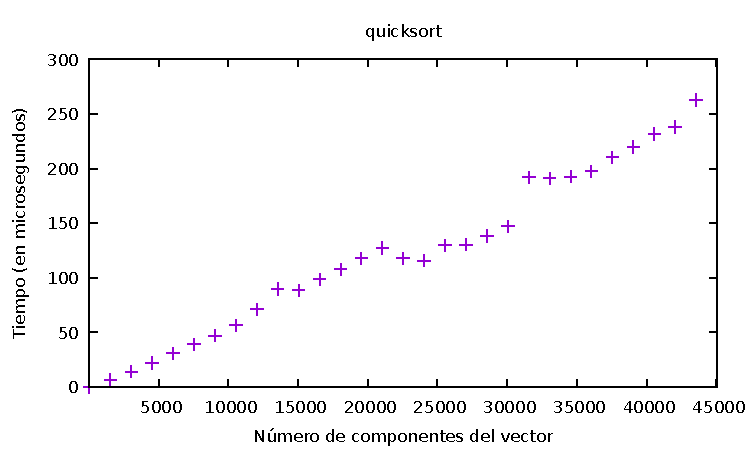
\includegraphics[width=0.7\textwidth]{../data/asus/quicksort-points.pdf}}

         \subfloat[HP]{
          \label{hp:quicksort-emp}
           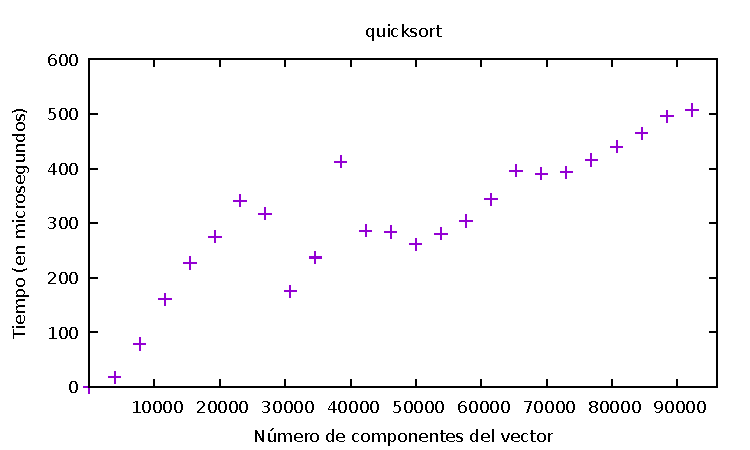
\includegraphics[width=0.7\textwidth]{../data/hp/quicksort-points.pdf}}

         \subfloat[LENOVO]{
          \label{lenovo:qicksort-emp}
           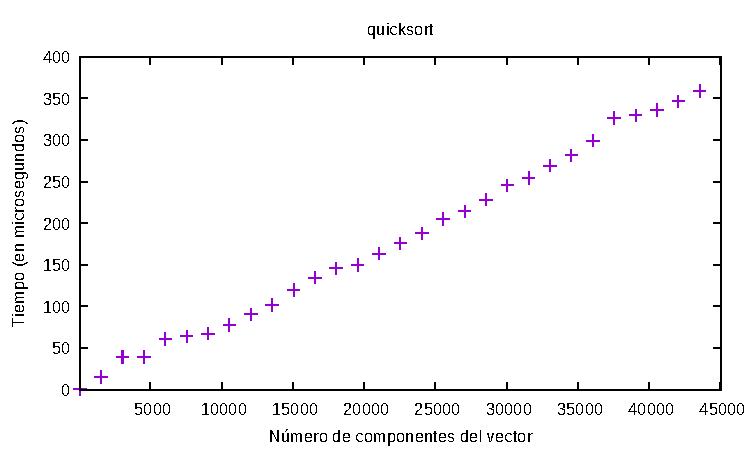
\includegraphics[width=0.7\textwidth]{../data/lenovo/quicksort-points.pdf}}
        \caption{Representación gráfica de tiempos de ejecución del algoritmo de ordenación QuickSort.}

        \label{emp:quicksort}
    \end{figure}

    

    \newpage
    
    \subsection{Algoritmo de inserción}
    
    En la siguiente tabla se encuentran los datos obtenidos en este algoritmo por cada uno de los
    equipos en los que hemos ejecutado el algoritmo. 
    
    \begin{table}[h]
        \footnotesize
        \centering
        \begin{tabular}{|r|r|r|r|}
            \hline
            \text{$N_{componentes}$} & \text{$t_{ASUS}$} & \text{$t_{HP}$} & \text{$t_{LENOVO}$} \\
            \hline
            50 & 0.14 & 0.17 & 0.33 \\ 
            4048 & 453.56 & 515.99 & 651.62 \\ 
            8046 & 1754.95 & 1812.13 & 2302.02 \\ 
            12044 & 3939.03 & 3964.86 & 5151.86 \\ 
            16042 & 7001.02 & 7121.99 & 9086.88 \\ 
            20040 & 10881.51 & 11267.74 & 14199.60 \\ 
            24038 & 15631.83 & 16306.35 & 20487.40 \\ 
            28036 & 21153.50 & 22116.26 & 27616.21 \\ 
            32034 & 27637.29 & 28858.12 & 36049.05 \\ 
            36032 & 34987.36 & 36138.26 & 45555.31 \\ 
            40030 & 43165.74 & 44968.61 & 55917.47 \\ 
            44028 & 52206.10 & 54424.15 & 67842.75 \\ 
            48026 & 62037.85 & 64616.22 & 80669.90 \\ 
            52024 & 72855.27 & 75586.21 & 94386.29 \\ 
            56022 & 84416.77 & 86679.96 & 109490.70 \\ 
            60020 & 97044.37 & 98427.26 & 125816.55 \\ 
            64018 & 110296.65 & 112276.70 & 143332.05 \\ 
            68016 & 124351.80 & 125903.00 & 161613.60 \\ 
            72014 & 139565.40 & 140651.00 & 180965.90 \\ 
            76012 & 155826.80 & 154545.50 & 201664.70 \\ 
            80010 & 172265.90 & 171206.85 & 223414.75 \\ 
            84008 & 189906.35 & 187602.35 & 246361.85 \\ 
            88006 & 208708.60 & 206964.30 & 269969.40 \\ 
            92004 & 228250.85 & 229561.45 & 295370.30 \\ 
            96002 & 248827.55 & 245400.70 & 321198.25 \\ 
            \hline
        \end{tabular}
        \caption{Tiempos de ejecución (en $\mu$s) del algoritmo de inserción}
    \end{table}

    Tal y como podemos observar, tenemos que nuevamente el equipo de ASUS ofrece un \textbf{mejor rendimiento} respecto a los otros
    dos equipos en los que se ha realizado el análisis. Asimismo, el tiempo de ejecución aumenta considerablemente
    en cuanto el número de componentes de vector en comparación con los algoritmos de QuickSort o MergeSort. 

    \begin{figure}[h]
        \centering
        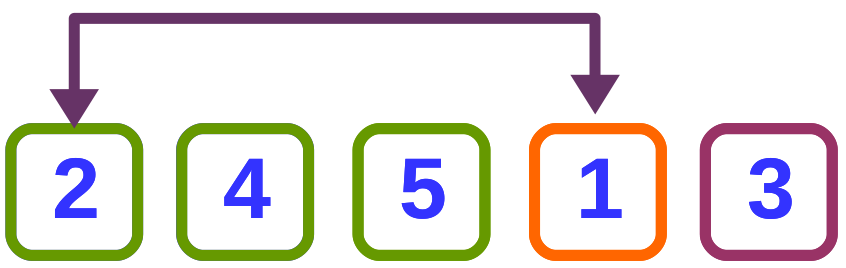
\includegraphics[width=0.5\textwidth]{img/insercion.png}
        \caption{Ilustración del funcionamiento interno del algoritmo de inserción}
    \end{figure}

    Las gráficas asociadas a cada equipo se pueden encontrar a continuación:

    \begin{figure}
        \centering
         \subfloat[ASUS]{
          \label{asus:insercion-emp}
           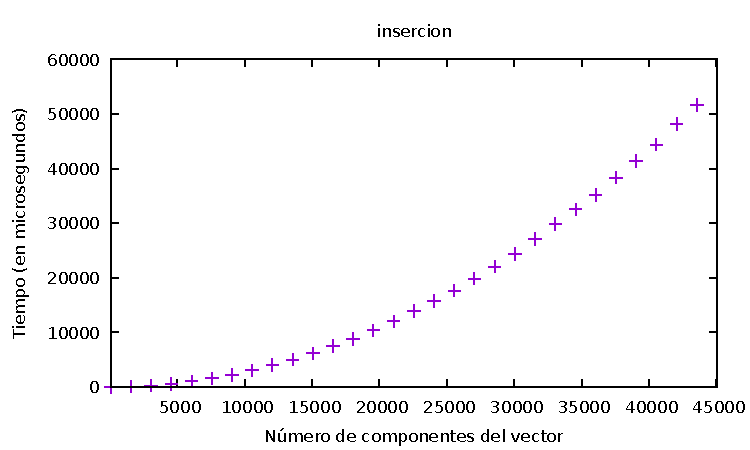
\includegraphics[width=0.7\textwidth]{../data/asus/insercion-points.pdf}}

         \subfloat[HP]{
          \label{hp:insercion-emp}
           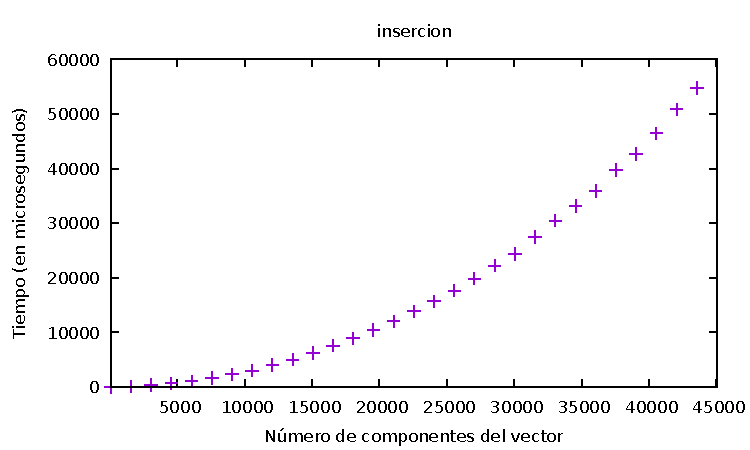
\includegraphics[width=0.7\textwidth]{../data/hp/insercion-points.pdf}}

         \subfloat[LENOVO]{
          \label{lenovo:insercion-emp}
           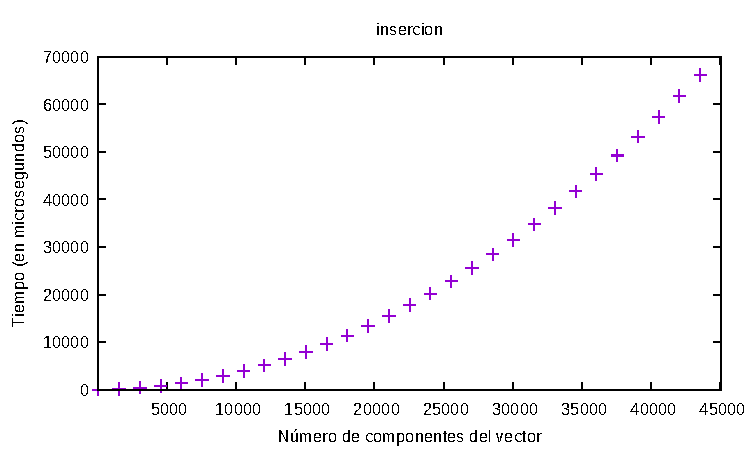
\includegraphics[width=0.7\textwidth]{../data/lenovo/insercion-points.pdf}}
        \caption{Representación gráfica de tiempos de ejecución del algoritmo de inserción.}

        \label{emp:insercion}
    \end{figure}
    
    \newpage 
    
    \subsection{Algoritmo de Floyd}

    En la siguiente tabla se encuentran los datos obtenidos en este algoritmo por cada uno de los
    equipos en los que hemos ejecutado el algoritmo. 

    \begin{table}[h]
        \centering
        \begin{tabular}{|r|r|r|r|}
            \hline
            \text{$N_{nod}$} & \text{$t_{ASUS}$} & \text{$t_{HP}$} & \text{$t_{LENOVO}$} \\
            \hline
            5 & 0.09 & 0.10 & 0.13 \\ 
            35 & 4.63 & 5.04 & 3.79 \\ 
            65 & 28.11 & 36.27 & 22.68 \\ 
            95 & 98.97 & 59.42 & 76.20 \\ 
            125 & 206.65 & 291.02 & 171.84 \\ 
            155 & 250.74 & 340.20 & 294.25 \\ 
            185 & 368.58 & 490.17 & 466.89 \\ 
            215 & 572.04 & 588.29 & 727.49 \\ 
            245 & 846.54 & 873.17 & 1069.24 \\ 
            275 & 1193.13 & 1234.56 & 1530.57 \\ 
            305 & 1642.20 & 1666.67 & 2058.39 \\ 
            335 & 2164.11 & 2205.70 & 2755.76 \\ 
            365 & 2826.06 & 2846.01 & 3574.31 \\ 
            395 & 3528.34 & 3583.40 & 4484.65 \\ 
            425 & 4410.26 & 4465.64 & 5606.11 \\ 
            455 & 5383.56 & 5485.51 & 6820.05 \\ 
            485 & 6554.77 & 6483.90 & 8154.31 \\ 
            515 & 7855.67 & 7928.90 & 9760.62 \\ 
            545 & 9386.40 & 9268.55 & 11542.12 \\ 
            575 & 10957.08 & 10777.34 & 13740.25 \\ 
            605 & 12786.02 & 12425.00 & 15864.58 \\ 
            635 & 14618.06 & 14709.94 & 18181.38 \\ 
            665 & 16823.92 & 16768.84 & 21031.77 \\ 
            695 & 19147.07 & 18815.95 & 23953.15 \\ 
            725 & 21807.53 & 21948.21 & 27128.60 \\ 
            \hline
        \end{tabular}
        \caption{Tiempos de ejecución (en $\mu$s) del algoritmo de Floyd}
    \end{table}

    En concordancia con los resultados obtenidos en las anteriores tablas, el ordenador que ofrece peores
    tiempos es el LENOVO, siendo el de ASUS el que ofrece resultados con mayor rapidez. 

    \begin{figure}[h]
        \centering
        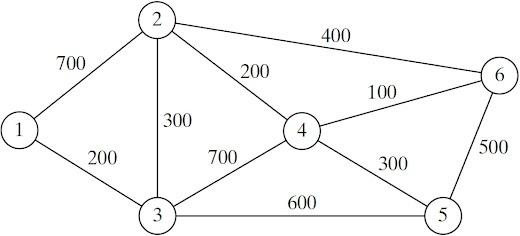
\includegraphics[width=0.4\textwidth]{img/graf-floyd.jpeg}
        \caption{Representacion gráfica de un grafo.}
    \end{figure}

    % \begin{figure}
    %     \centering
    %      \subfloat[ASUS]{
    %       \label{asus:floyd-emp}
    %        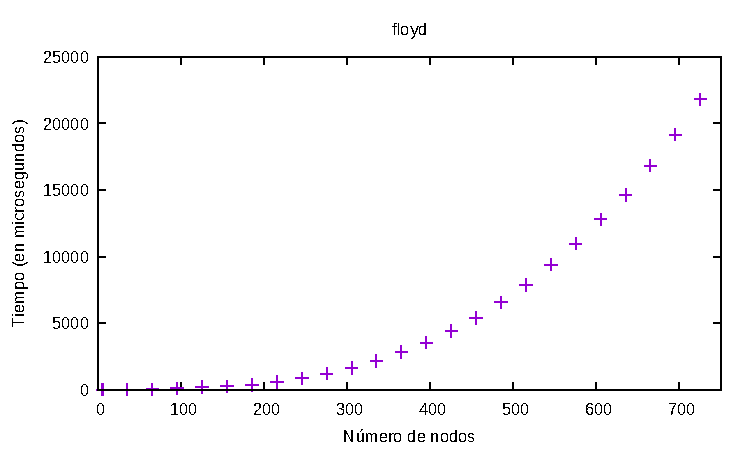
\includegraphics[width=0.7\textwidth]{../data/asus/floyd-points.pdf}}

    %      \subfloat[HP]{
    %       \label{hp:floyd-emp}
    %        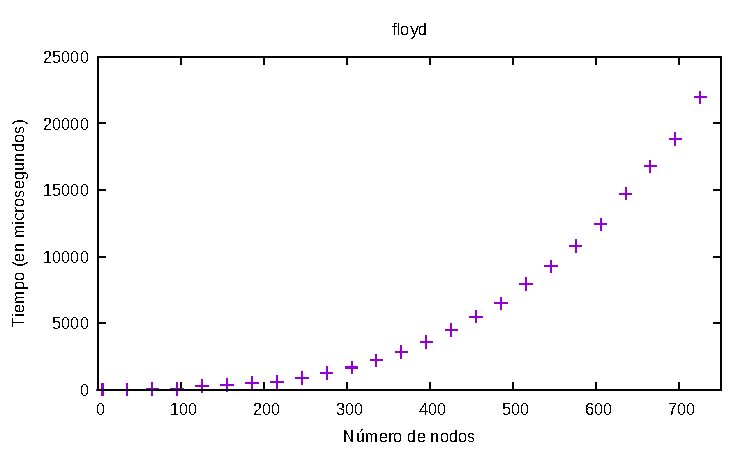
\includegraphics[width=0.7\textwidth]{../data/hp/floyd-points.pdf}}

    %      \subfloat[LENOVO]{
    %       \label{lenovo:floyd-emp}
    %        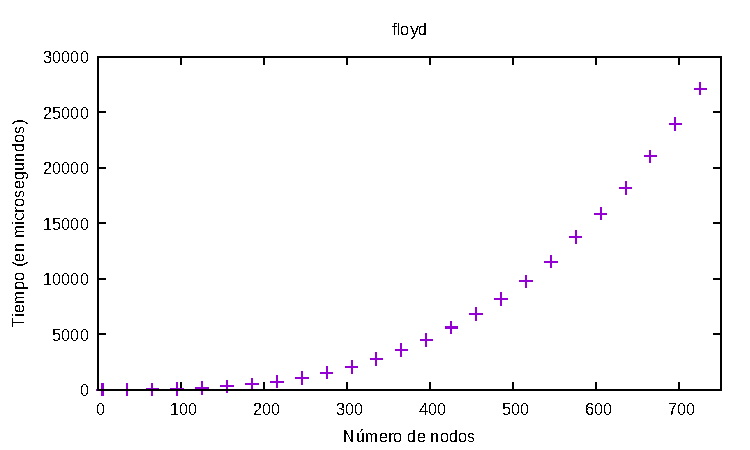
\includegraphics[width=0.7\textwidth]{../data/lenovo/floyd-points.pdf}}
    %     \caption{Representación gráfica de tiempos de ejecución del algoritmo Floyd.}

    %     \label{emp:floyd}
    % \end{figure}
    
    \subsection{Algoritmo Hanoi}

    En la siguiente tabla se encuentran los datos obtenidos en este algoritmo por cada uno de los
    equipos en los que hemos ejecutado el algoritmo. 

    \begin{table}[h]
        \centering
        \begin{tabular}{|r|r|r|r|}
            \hline
            \text{$N_{disk}$} & \text{$t_{ASUS}$} & \text{$t_{HP}$} & \text{$t_{LENOVO}$} \\
            \hline
            2 & 0.04 & 0.10 & 0.16 \\ 
            3 & 0.08 & 0.10 & 0.20 \\ 
            4 & 0.08 & 0.14 & 0.20 \\ 
            6 & 0.08 & 0.42 & 0.22 \\ 
            7 & 0.24 & 0.36 & 0.26 \\ 
            8 & 0.18 & 0.50 & 0.48 \\ 
            10 & 0.22 & 0.84 & 0.52 \\ 
            11 & 0.36 & 1.22 & 0.74 \\ 
            12 & 1.10 & 3.90 & 1.88 \\ 
            13 & 2.38 & 6.52 & 4.06 \\ 
            14 & 5.26 & 6.26 & 6.98 \\ 
            16 & 10.40 & 11.82 & 14.02 \\ 
            17 & 41.72 & 47.08 & 51.68 \\ 
            18 & 83.38 & 97.78 & 101.66 \\ 
            20 & 170.68 & 313.84 & 199.10 \\ 
            21 & 340.14 & 494.60 & 373.10 \\ 
            22 & 1185.76 & 1084.10 & 1605.38 \\ 
            23 & 1776.36 & 2082.46 & 2712.62 \\ 
            24 & 3295.08 & 3465.74 & 4693.84 \\ 
            26 & 6642.10 & 6844.50 & 9232.04 \\ 
            \hline
        \end{tabular}
        \caption{Tiempos de ejecución (en $\mu$s) del algoritmo de Floyd}
    \end{table}

    Así que como preveíamos, puesto que habíamos estudiado las características de cada ordenador, hemos visto que el ASUS al 
    tener un i7 de 10ª generación ejecuta más rápido el algoritmo, mientras que el LENOVO es el computador que más tarda, 
    lógicamente al tratarse de un i5.

    \begin{figure}[h]
        \centering
        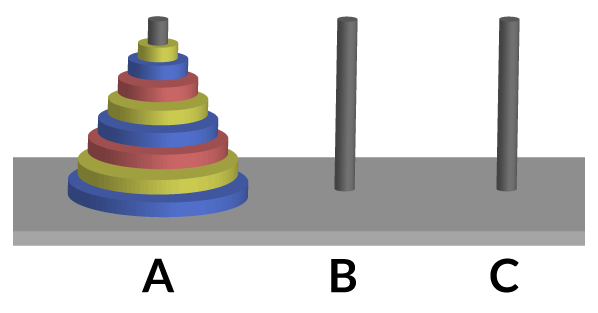
\includegraphics[width=0.4\textwidth]{img/hanoi.png}
        \caption{Representacion gráfica del juego de las Torres de Hanoi.}
    \end{figure}

    Ahora vamos a mostrar las gráficas resultantes tras calcular el tiempo que tarda la ejecución de este algoritmo para diferentes
    tamaños, en este caso, para distinto número de discos.

    \begin{figure}
        \centering
         \subfloat[ASUS]{
          \label{asus:hanoi-emp}
           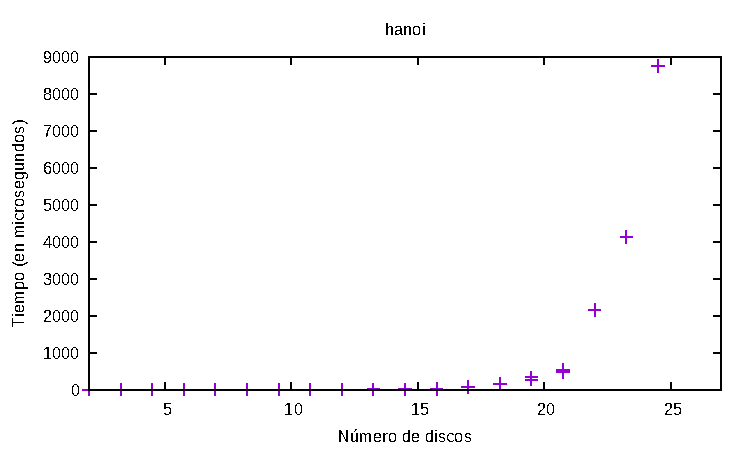
\includegraphics[width=0.7\textwidth]{../data/asus/hanoi-points.pdf}}

         \subfloat[HP]{
          \label{hp:hanoi-emp}
           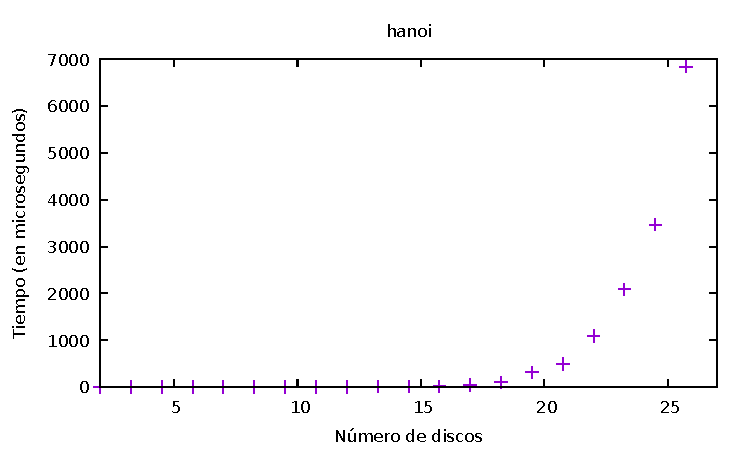
\includegraphics[width=0.7\textwidth]{../data/hp/hanoi-points.pdf}}

         \subfloat[LENOVO]{
          \label{lenovo:hanoi-emp}
           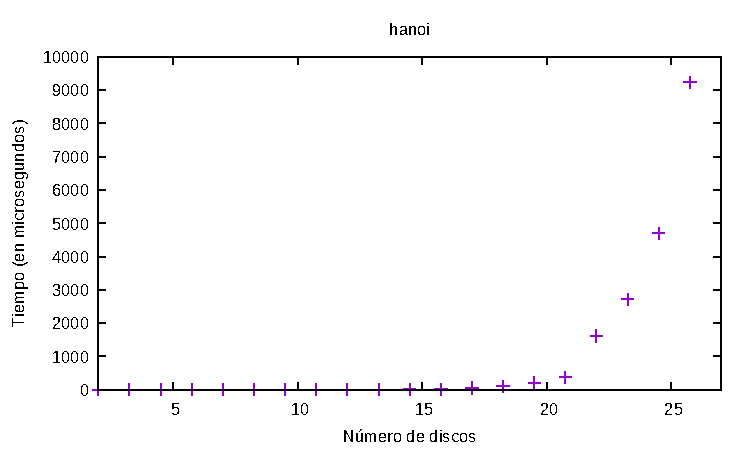
\includegraphics[width=0.7\textwidth]{../data/lenovo/hanoi-points.pdf}}
        \caption{Representación gráfica de tiempos de ejecución del algoritmo de resolución del juego de las Torres de Hanoi.}

        \label{emp:hanoi}
    \end{figure}

    \section{Comparación de ejecuciones con diferentes niveles de optimización}

    \subsection{Conceptos teóricas}

    A continuación, usaremos el algoritmo de Floyd para ilustrar uno de los objetivos mencionados de la práctica, 
    el cual consiste en analizar la eficiencia de un mismo algoritmo para optimizaciones del compilador diferentes.
    En concreto, al igual que en el resto de ejecuciones, usamos g++ como compilador, y analizaremos las siguientes
    opciones de optimización:

    \begin{itemize}
        \item \textbf{-O0 (sin optimización)}: Desconecta por completo la optimización y es el predeterminado si 
        no se especifica ningún nivel.
        \item \textbf{-O1}: El nivel de optimización más básico. El compilador intentará producir un código rápido
        y pequeño sin tomar mucho tiempo de compilación. 
        \item \textbf{-O2}: Un paso delante de -O1. Es el nivel recomendado de optimización, a no ser que el sistema
        tenga necesidades especiales. -O2 activará algunas opciones añadidas a las que se activan con -O1. 
        Con -O2, el compilador intentará aumentar el rendimiento del código sin comprometer el tamaño y sin tomar 
        mucho más tiempo de compilación.
        \item \textbf{-O3}:  El nivel más alto de optimización posible. Activa optimizaciones que son caras en términos 
        de tiempo de compilación y uso de memoria. El hecho de compilar con -O3 no garantiza una forma de mejorar el 
        rendimiento y, de hecho, en muchos casos puede ralentizar un sistema debido al uso de binarios de gran tamaño y 
        mucho uso de la memoria.
    \end{itemize} 
    
    \subsection{Tablas de ejecución} 

    Los tiempos de ejecución para los diferentes niveles de optimización se presentan en la siguiente tabla. 

    \begin{table}[H]
        \centering
        \begin{tabular}{|r|r|r|r|r|}
            \hline
            $N_{nodos}$ & $T_{O0}$ & $T_{O1}$ & $T_{O2}$ & $T_{O3}$ \\
            \hline
            5 & 0.17 & 0.08 & 0.06 & 0.07 \\ 
            35 & 53.95 & 4.47 & 3.02 & 3.52 \\ 
            65 & 380.01 & 27.30 & 26.04 & 35.80 \\ 
            95 & 490.60 & 92.52 & 124.14 & 127.20 \\ 
            125 & 841.45 & 205.10 & 275.73 & 198.03 \\ 
            155 & 1494.98 & 386.86 & 360.05 & 219.22 \\ 
            185 & 2494.07 & 447.26 & 367.53 & 368.06 \\ 
            215 & 3892.51 & 688.94 & 564.97 & 573.63 \\ 
            245 & 5761.86 & 1032.51 & 849.70 & 843.58 \\ 
            275 & 8168.23 & 1443.59 & 1183.75 & 1205.76 \\ 
            305 & 10994.11 & 1997.49 & 1617.42 & 1629.11 \\ 
            335 & 14597.46 & 2648.92 & 2166.47 & 2158.78 \\ 
            365 & 19297.67 & 3386.93 & 2794.19 & 2793.36 \\ 
            395 & 24360.22 & 4255.16 & 3517.28 & 3520.41 \\ 
            425 & 30149.47 & 5370.36 & 4386.85 & 4494.97 \\ 
            455 & 37490.57 & 6552.51 & 5482.11 & 5511.59 \\ 
            485 & 46042.69 & 7993.95 & 6694.07 & 6717.87 \\ 
            515 & 53611.57 & 9620.67 & 7998.24 & 7933.97 \\ 
            545 & 63969.28 & 11346.75 & 9421.14 & 9432.59 \\ 
            575 & 76580.04 & 13442.25 & 11065.08 & 11010.14 \\ 
            605 & 87898.27 & 15581.91 & 12906.25 & 12797.45 \\ 
            635 & 102621.15 & 18516.74 & 14833.09 & 14603.30 \\ 
            665 & 117634.85 & 21025.31 & 16875.94 & 16933.83 \\ 
            695 & 133193.50 & 23857.43 & 19786.48 & 19152.38 \\ 
            725 & 152998.80 & 27005.65 & 22494.99 & 22495.65 \\ 
            \hline
        \end{tabular}
        \caption{Tiempos de ejecución (en $\mu$s) para algoritmo Floyd (Asus)}
    \end{table}

    \begin{figure}[H]
        \centering
        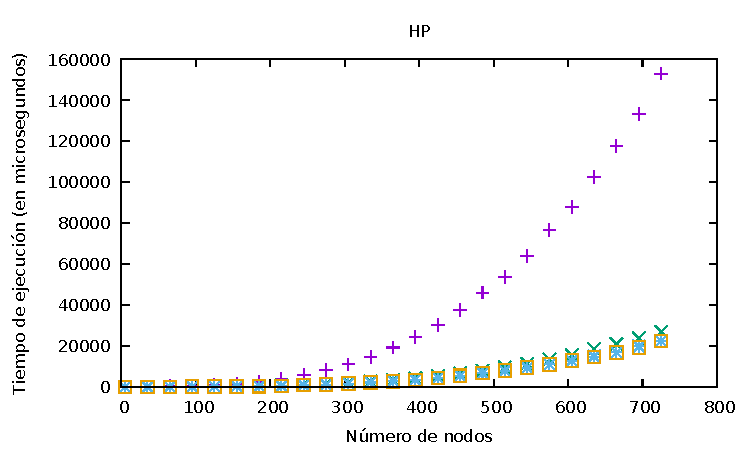
\includegraphics[width=0.6\textwidth]{../data/asus-opt.pdf}
        \caption{Gráfica de tiempos de ejecución (Asus)}
    \end{figure}

    \begin{table}[H]
        \centering
        \begin{tabular}{|r|r|r|r|r|}
            \hline
            $N_{nodos}$ & $T_{O0}$ & $T_{O1}$ & $T_{O2}$ & $T_{O3}$ \\
            \hline
            5 & 0.21 & 0.10 & 0.09 & 0.10 \\ 
            35 & 39.48 & 3.78 & 6.07 & 5.20 \\ 
            65 & 251.96 & 46.40 & 48.65 & 42.72 \\ 
            95 & 574.10 & 179.56 & 146.43 & 145.99 \\ 
            125 & 793.83 & 301.52 & 266.95 & 175.65 \\ 
            155 & 1510.12 & 286.76 & 318.89 & 309.46 \\ 
            185 & 2495.91 & 449.75 & 376.88 & 404.58 \\ 
            215 & 3914.89 & 708.44 & 577.90 & 586.26 \\ 
            245 & 5701.98 & 1028.52 & 853.82 & 875.53 \\ 
            275 & 8082.82 & 1492.51 & 1207.13 & 1231.23 \\ 
            305 & 10928.36 & 1971.31 & 1638.46 & 1670.67 \\ 
            335 & 14455.55 & 2698.91 & 2178.86 & 2174.05 \\ 
            365 & 18929.88 & 3473.24 & 2837.69 & 2833.66 \\ 
            395 & 24332.74 & 4414.80 & 3564.82 & 3646.11 \\ 
            425 & 29848.49 & 5443.34 & 4421.02 & 4510.19 \\ 
            455 & 36908.89 & 6591.26 & 5360.57 & 5432.05 \\ 
            485 & 44582.97 & 8053.35 & 6493.54 & 6667.46 \\ 
            515 & 53470.68 & 9527.39 & 7778.40 & 7889.72 \\ 
            545 & 63172.00 & 11443.67 & 9345.16 & 9462.12 \\ 
            575 & 75819.62 & 13436.56 & 10767.32 & 10656.11 \\ 
            605 & 86390.05 & 15466.07 & 12933.42 & 12717.99 \\ 
            635 & 100187.65 & 17941.33 & 14708.66 & 14143.55 \\ 
            665 & 117042.70 & 20676.88 & 16400.16 & 16729.92 \\ 
            695 & 131518.20 & 23515.96 & 18637.03 & 19198.70 \\ 
            725 & 147998.15 & 26638.71 & 21326.99 & 21331.96 \\ 
            \hline
        \end{tabular}
        \caption{Tiempos de ejecución (en $\mu$s) para algoritmo Floyd (HP)}
    \end{table}

    \begin{figure}[H]
        \centering
        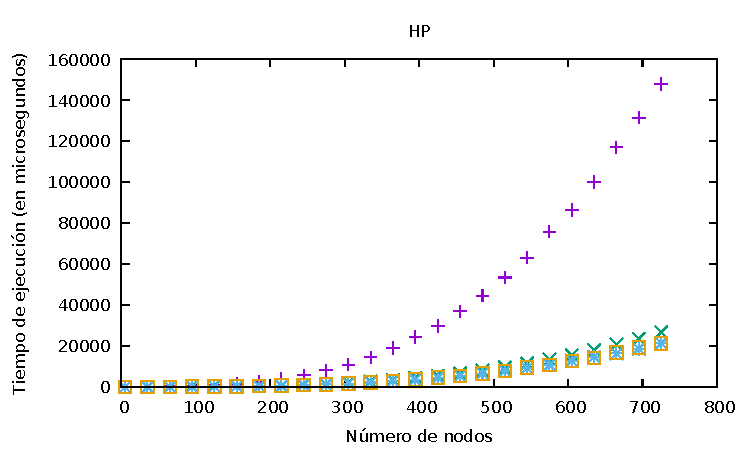
\includegraphics[width=0.6\textwidth]{../data/hp_opt.pdf}
        \caption{Gráfica de tiempos de ejecución (HP)}
    \end{figure}


    \begin{table}[H]
        \centering
        \begin{tabular}{|r|r|r|r|r|}
            \hline
            $N_{nodos}$ & $T_{O0}$ & $T_{O1}$ & $T_{O2}$ & $T_{O3}$ \\
            \hline
            5 & 0.23 & 0.17 & 0.23 & 0.33 \\ 
            35 & 29.84 & 6.48 & 5.50 & 5.55 \\ 
            65 & 203.45 & 35.44 & 31.70 & 37.05 \\ 
            95 & 645.68 & 135.50 & 126.25 & 116.51 \\ 
            125 & 1138.86 & 294.69 & 266.38 & 199.54 \\ 
            155 & 2220.49 & 530.83 & 466.20 & 370.52 \\ 
            185 & 3524.26 & 866.54 & 794.60 & 661.22 \\ 
            215 & 5531.06 & 1340.55 & 1108.49 & 1120.88 \\ 
            245 & 9879.07 & 2039.46 & 1490.56 & 1765.31 \\ 
            275 & 14760.01 & 2775.61 & 1988.81 & 2839.12 \\ 
            305 & 21002.12 & 3709.97 & 2736.05 & 2645.93 \\ 
            335 & 21130.67 & 4774.23 & 3574.84 & 4324.62 \\ 
            365 & 28563.90 & 5061.25 & 4065.97 & 4587.72 \\ 
            395 & 35266.89 & 7312.15 & 5092.35 & 6049.83 \\ 
            425 & 43856.27 & 9466.16 & 6145.76 & 7357.14 \\ 
            455 & 63704.19 & 11719.27 & 8768.52 & 9735.48 \\ 
            485 & 71028.24 & 15156.26 & 10372.40 & 9273.38 \\ 
            515 & 85424.65 & 24115.51 & 13265.73 & 11000.40 \\ 
            545 & 103213.98 & 16958.10 & 14592.08 & 12854.59 \\ 
            575 & 123200.59 & 18765.49 & 15596.62 & 24142.65 \\ 
            605 & 134205.15 & 20772.30 & 17569.12 & 29495.03 \\ 
            635 & 197191.95 & 31057.76 & 20804.73 & 34560.04 \\ 
            665 & 224866.25 & 27874.88 & 28951.74 & 32018.41 \\ 
            695 & 203138.40 & 35154.18 & 46677.95 & 27752.09 \\ 
            725 & 214510.65 & 50098.56 & 40081.61 & 35497.00 \\ 
            \hline
        \end{tabular}
        \caption{Tiempos de ejecución (en $\mu$s) para algoritmo Floyd (Lenovo)}
    \end{table}

    \begin{figure}[H]
        \centering
        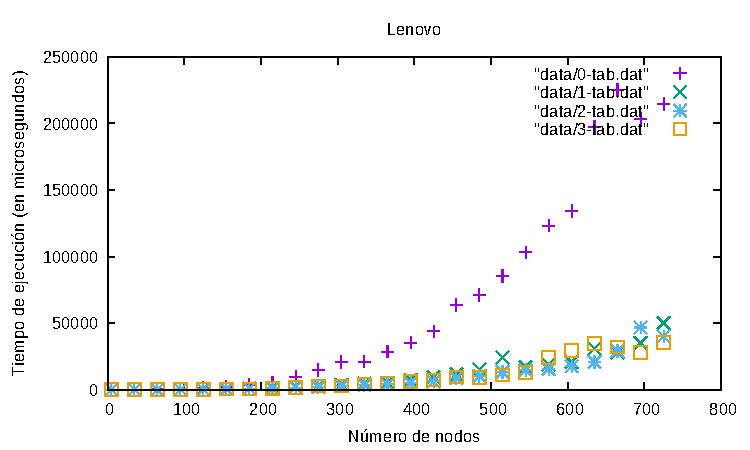
\includegraphics[width=0.6\textwidth]{../data/lenovo-opt.pdf}
        \caption{Gráfica de tiempos de ejecución (Lenovo)}
    \end{figure}

    \subsection{Observaciones}

    Observando las gráficas se puede apreciar que, para pequeños valores del número de nodos, las diferencias entre los
    tiempos de ejecución para diferentes niveles de optimización son prácticamente despreciables. Sin embargo, a medida
    que va aumentando la complejidad del grafo, los tiempos de ejecución para diferentes niveles de optimización se hacen
    más significativos, siendo que para el valor $n=725$, el algoritmo optimizado es prácticamente el cuádruple de rápido que
    el algoritmo sin optimizar. 

    Por tanto, concluimos que, para ejecuciones de tamaños pequeños, las diferencias son apenas apreciables, mientras que
    para grandes valores la optimización sí que puede aumentar considerablemente los tiempos de ejecución. Se trata, por
    consiguiente, de un buen mecanismo de optimización del código. 


    \section{Comparación de los algoritmos de ordenación}

    \subsection{Objetivos}

    En esta sección compararemos los algoritmos de ordenación presentados previamente. El objetivo será
    sacar conclusiones relevantes relacionados con la adecuación de cada algoritmo a cada situación. 

    A continuación se presentan los tiempos de ejecución de cada algoritmo en cada equipo en los que se ha realizado
    esta experiencia. 

    \section{Eficiencia híbrida}
    
    En esta sección trataremos los datos obtenidos de la sección anterior mediante técnicas estadísticas para
    comprobar la consistencia de los datos experimentales con los calculados teóricamente. 

    \subsection{Algoritmo de inserción}

    Las gráficas con las curvas de regresión son las siguientes:

    \begin{figure}[h]
        \centering
         \subfloat[ASUS]{
          \label{asus:insercion-hib}
           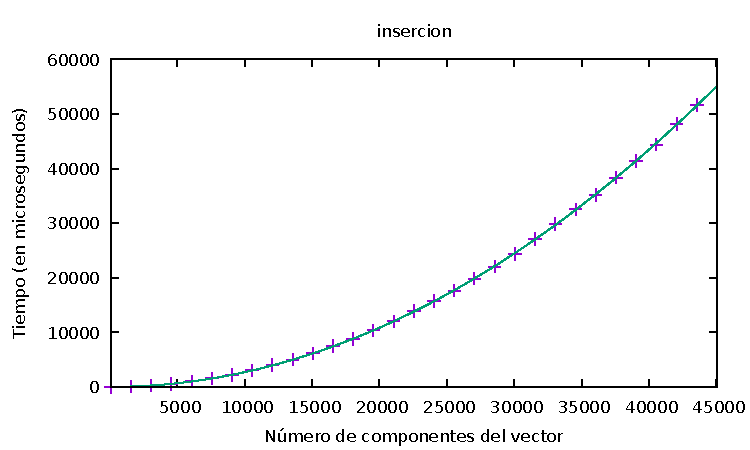
\includegraphics[width=0.7\textwidth]{../data/asus/insercion-graph.pdf}}

         \subfloat[HP]{
          \label{hp:insercion-hib}
           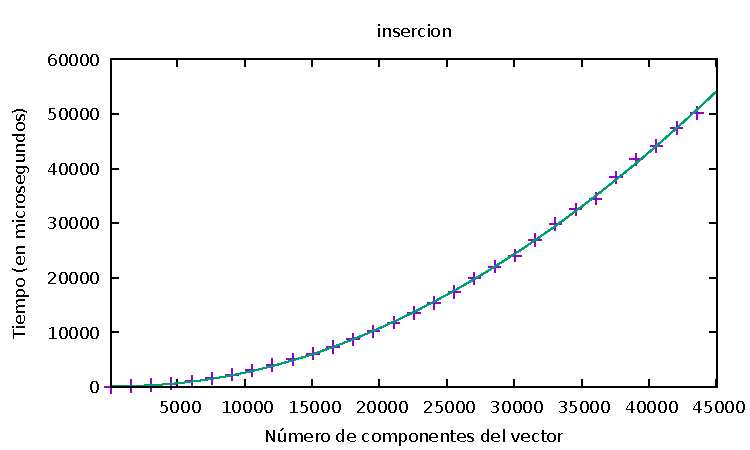
\includegraphics[width=0.7\textwidth]{../data/hp/insercion-graph.pdf}}

         \subfloat[LENOVO]{
          \label{lenovo:insercion-hib}
           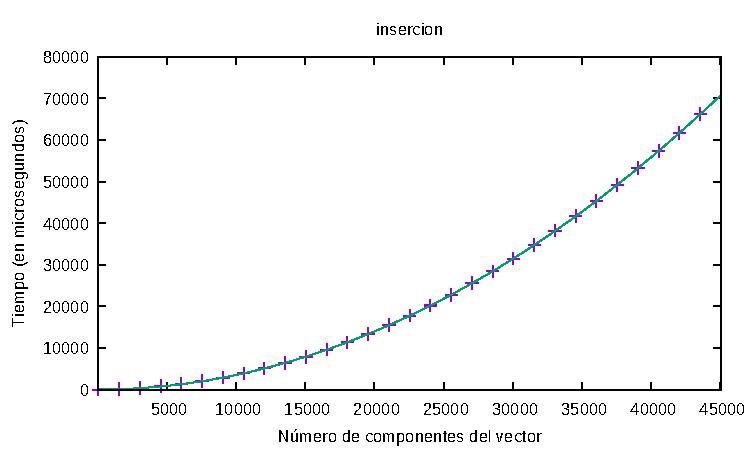
\includegraphics[width=0.7\textwidth]{../data/lenovo/insercion-graph.pdf}}
        \caption{Gráficas de regresión de los algoritmos de inserción.}

        \label{hib:insercion}
    \end{figure}

    Para cada una de ellas se han obtenido los siguientes datos:

    \begin{itemize}

        \item \textbf{Asus}
            \begin{itemize}
                \item Mejor funcion de ajuste: $ $
            \end{itemize}
        \item 

        \item \textbf{HP}
            \begin{itemize}
                \item Mejor funcion de ajuste
            \end{itemize}
        \item 

        \item \textbf{Lenovo}
            \begin{itemize}
                \item Mejor funcion de ajuste
            \end{itemize}
        \item 

        
    \end{itemize}

    % \subsection{Algoritmo HeapSort}
    % \subsection{Algoritmo QuickSort}
    % \subsection{Algoritmo de Floyd}
    
\end{document}